\documentclass[utf8]{ctexart}


\usepackage{amssymb}
\usepackage{enumerate}
\usepackage[numbers]{natbib} 
\usepackage{geometry}
\geometry{left=3.0cm,right=3.0cm,top=2.5cm,bottom=2.5cm}
\usepackage{fancyhdr}
\usepackage{wrapfig}
\usepackage{subfigure}
\pagestyle{fancy}
\lhead{}
\rhead{}
\setlength{\headheight}{10mm}
\fancyhead[C]{
	\begingroup
	\setlength{\tabcolsep}{10pt} % Default value: 6pt
	\renewcommand{\arraystretch}{1.5} % Default value: 1
	\begin{tabular}{ccc}
		& \large{\textbf{单色仪的定标和光谱测量实验报告}} &  \\
		少年班学院 \qquad \qquad & 刘子安 PB20000069 & \qquad \today
	\end{tabular}
	\endgroup
}   %在此处插入作者信息,改变页眉,此页眉是由我设计的,类似于实验报告纸
\fancyfoot[C]{ 第 {\thepage} 页,共 \pageref{unknown} 页}
\renewcommand{\headrulewidth}{0pt}


\usepackage{graphicx}
\graphicspath{{./Figure/}}
\usepackage{siunitx}

\begin{document}
	
	\section*{实验目的}
	\begin{enumerate}
		\item 
		了解光栅单色仪的结构以及工作原理并熟练掌握其使用方法
		\item 
		掌握调节光路准直的基本方法和技巧,利用钠灯等标准光源对单色仪进行定标
		\item 
		测量红宝石的发射光谱,加深对物质发光光谱特性的了解
	\end{enumerate}
	
	\section*{实验方法}
	\subsection*{实验仪器}
	WDS-8 型组合式多功能光栅光谱仪,具体参数:焦距 f=500 
	mm.光栅条数:1200 gr/mm。狭缝宽度在 0-2 mm 连续可调,示值精度 0.01 mm。光电
	倍增管的测量范围:200-800 nm;CCD 的测量范围:300-900 nm
	
	\subsection*{实验原理}
	光栅光谱仪是利用衍射作为色散元件,因此光栅作为分光器件就成为决定光栅光谱仪的性能的
	主要因素。
	\subsubsection*{1. 衍射光栅:}
	设有一束光以入射角$\theta_0$射向一块衍射光栅,则只有满足下式的一些特殊角度$\theta_m$下,才有光束衍射出来
	\begin{equation}
		d(\sin{\theta_0}\pm\sin{\theta_m})=m\lambda
	\end{equation}

	上式为著名的光栅方程,式中$\theta_0$为入射角,$\theta_m$为衍射角,$d$为光栅常数,$m=0,\pm1,\pm2,...$
	
	还可以推得光栅的分辨率为:
	\begin{equation}
		\frac{\Delta\lambda}{\lambda} = \frac{Nd}{\lambda}(\sin{\theta_0}+\sin{\theta_m})
	\end{equation}

	\subsubsection*{2. 闪耀光栅:}
	\begin{wrapfigure}{r}{8cm}
		\centering
		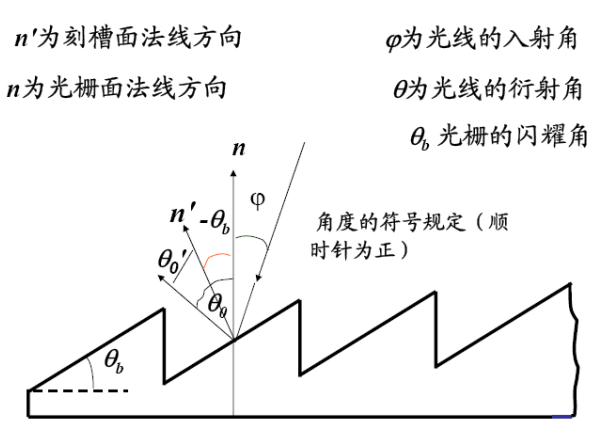
\includegraphics[scale=0.6]{Graph1.png}
		\caption{闪耀光栅}
	\end{wrapfigure}
	闪耀定义为将一段光谱的衍射最大转移到其他衍射阶次而非零阶。通过特殊设计,闪耀光栅能够实现在特定波长的最大衍射效率。一片光栅的闪耀波长取决于刻槽几何尺寸的选择。

	当入射光与光栅面的法线$n$的方向的夹角为$\phi$时,光栅的衍射角为$\theta_b$,取一级衍射项,对于入射角为$\phi$,而衍射角为$\theta$时,光栅方程为:
	\begin{equation}
		d(\sin{\phi}+\sin{\theta_m})=m\lambda
	\end{equation}
	
	\section*{实验记录及数据处理}
	\subsection*{实验数据及处理}
	\subsubsection*{1. 光谱单色仪的定标}
	在合适位置得到低压钠灯的双光谱线$(\qty{589.0}{nm}$和$\qty{589.6}{nm})$完全分离开的光谱曲线如图:
	\begin{figure}[htbp]
		\centering
		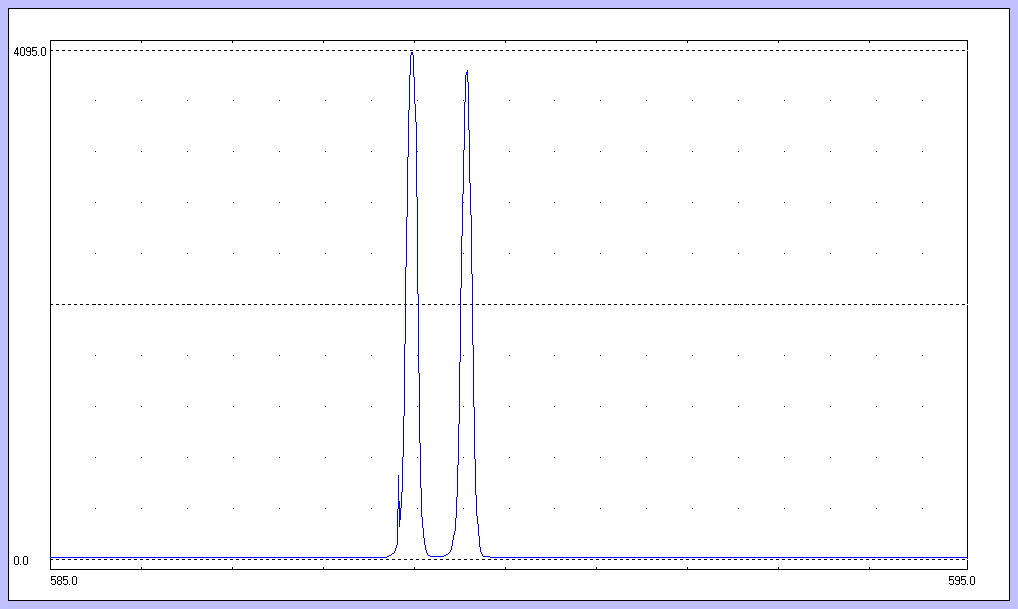
\includegraphics[scale=0.6]{1.png}
		\caption{钠光谱主线系}
	\end{figure}

	记录此时的负高压值为$-437V$,并定标。
	\subsubsection*{2.测量低压钠灯的光谱}
	调整仪器,测量锐线系的$\qty{615.4}{nm}$和$\qty{616.0}{nm}$曲线:
	\begin{figure}[htbp]
		\centering
		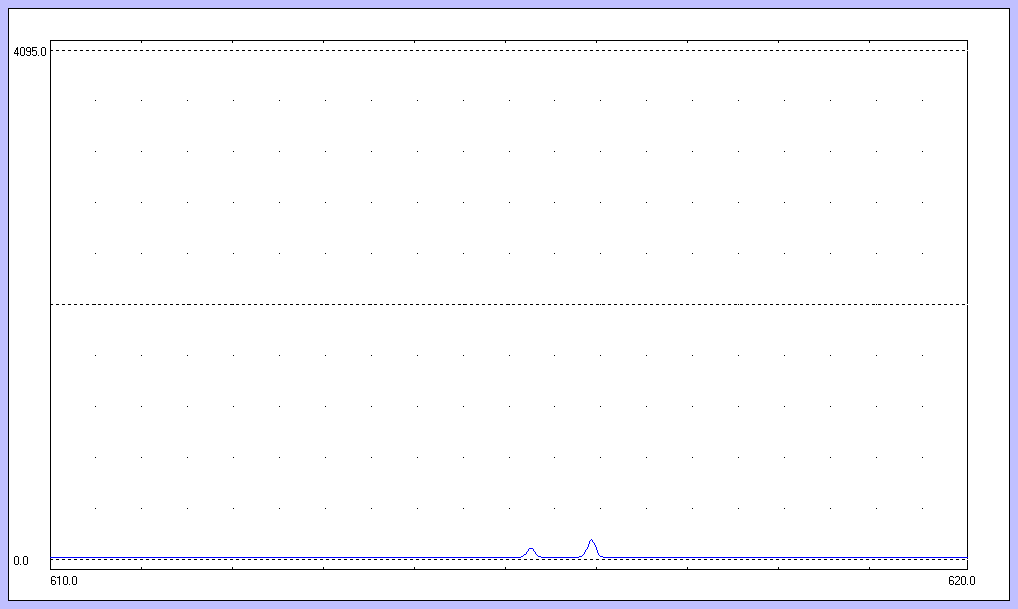
\includegraphics[scale=0.6]{3rui.png}
		\caption{钠光谱锐线系}
	\end{figure}

	从图中可以得到两条谱线的波长分别是$\qty{615.237}{nm}$和$\qty{615.900}{nm}$。
	
	再测量漫线系的两对谱线$\qty{568.3}{nm}$和$\qty{568.86}{nm}$,$\qty{497.78}{nm}$和$\qty{498.2}{nm}$:
	\begin{figure}[htbp]
		\centering
		\subfigure[第一组]{
		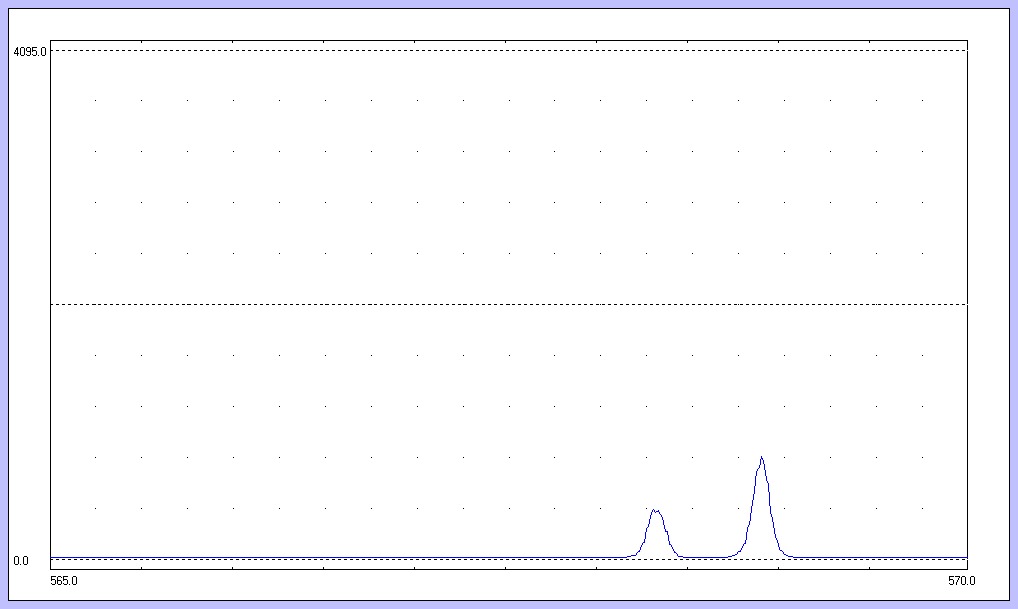
\includegraphics[scale=0.4]{4man.png}
	}
		\hspace{0.1in} %两图片距离
		\subfigure[第二组]{
		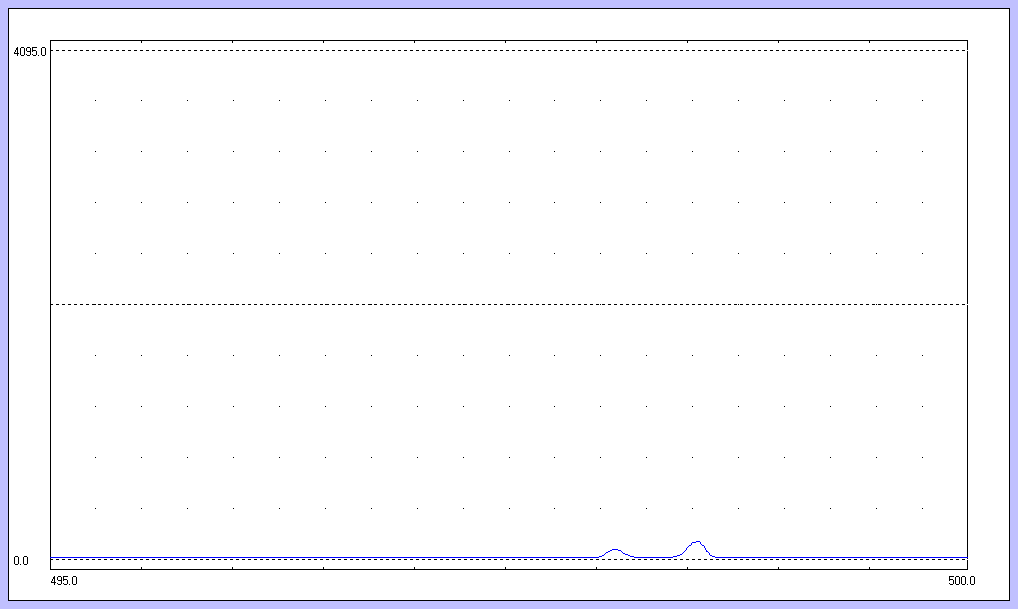
\includegraphics[scale=0.4]{5man.png}
	}
	\caption{钠光谱漫线系}
	\end{figure}

	读取测得数据中的值可以得到测得的波长分别为$\qty{568.288}{nm}$和$\qty{568.875}{nm}$,$\qty{498.075}{nm}$和$\qty{498.525}{nm}$。
	
	可以利用测得的数据来求钠原子的里德伯常数,我们取漫线系的第一组谱线:
	\begin{equation}
		\frac{1}{\bar{\lambda}} = R\left(\frac{1}{(3-\Delta{p})^2} - \frac{1}{(4 - \Delta{d})^2}\right)
	\end{equation}
	
	其中$\Delta{p} = 0.88$,$\Delta{d} = 0.01$,$\bar{\lambda} = \frac{568.288+568.875}{2} \unit{nm}= \qty{568.5815}{nm}$,代入(3)式可解得:
	\begin{equation}
		R = 1.099 \times 10^7 \unit{m^{-1}}
	\end{equation}
	与实际值$R = 1.09734 \times 10^7 \unit{m^{-1}}$非常接近。

	\subsubsection*{3.红宝石发射光谱的测量}
	调整光路和高负压值,测得红宝石的发射光谱:
	\begin{figure}[htbp]
		\centering
		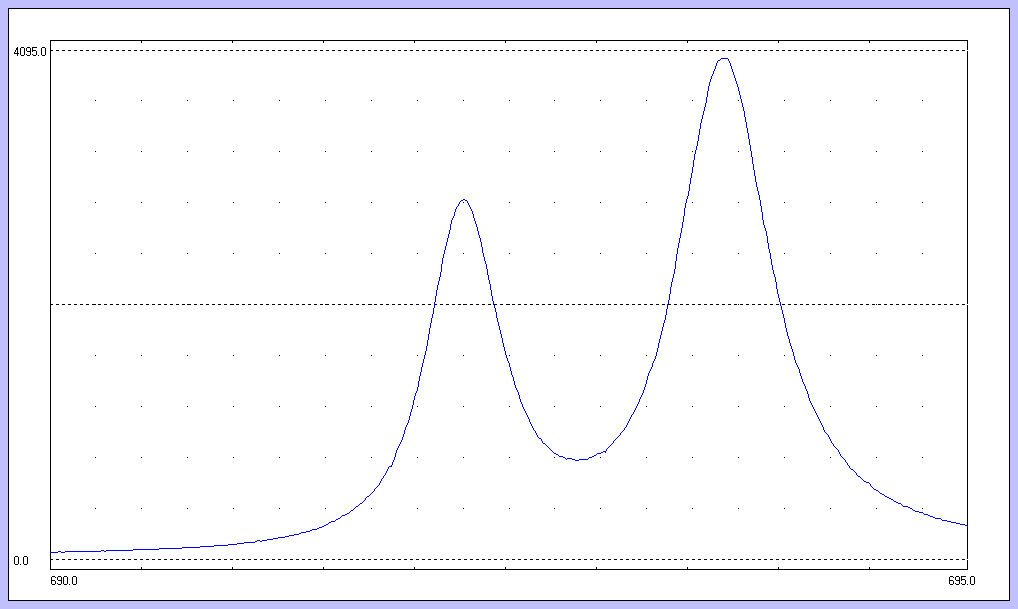
\includegraphics[scale=0.6]{6red.png}
		\caption{红宝石发射光谱}
	\end{figure}

	测得两个谱线的波长为$\qty{692.250}{nm}$和$\qty{693.675}{nm}$。
	
	\begin{itemize}
		\item [1.]红宝石发光原理\cite{art1}
		\par
		红宝石发光原理时光致发光。光致发光是指物质通过光激发产生的发光。物质的原子(离子)吸收激发光的能量变为激发态,从激发态返回到基态的过程中发出光。具体原理可参考文献\cite{art1}。
		\item [2.]红宝石发光应用
		
		用于制作激光器。红宝石激光器是世界上第一台制成的激光器,也是世界上最早应用于医疗领域的激光器,利用其波长特性广泛应用在各种色素性疾病;也可以用长脉冲模式用于永久性去除体毛;还可以利用调Q模式用于治疗蓝、黑和绿色文身以及各种良性色素性病变。在医疗领域还被应用在眼科,用于视网膜的焊接,治疗青光眼,虹膜的切除等。
		
		除了在医疗领域的应用,红宝石激光器也是很早就应用于军事以及全息成像等领域。1961年一台成为柯利达1号的红宝石激光测距机在美国诞生后,1962年第一台军用激光测距机便成功地进行了示范表演。
		
		
	\end{itemize}
	
	
	\subsection*{误差分析}
	本次实验主要误差应该来自于初始时定标的不够准确;系统的误差和测量时的误差。如强度过小或者噪音过多而导致读数不够准确。
		\subsection*{思考题}
	\begin{itemize}
		\item [1.] 如何求出入射狭缝的最佳宽度
		\item [ ]答:最佳狭缝宽度应该是 $a_n = 0.86\frac{\lambda f}{D}$
		\item [2.]单色仪的理论分辨本领如何计算?怎样测量单色仪的实际分辨本领?
		\item [ ]答:理论分辨本例为$R = \frac{\lambda}{\Delta\lambda} = Nm$,其中$N$为总刻线数,$m$为级数。实际则使用$R = \frac{\lambda}{\Delta\lambda}$,其中$\lambda = \frac{\lambda_1+\lambda_2}{2}$
	\end{itemize}
	
	\section*{结论}
	\subsection*{总结}
	本次实验总体做的比较成功,完成速度也比较快,最后尝试测量了红宝石的吸收曲线但是效果并不明显。
	
	\bibliographystyle{plain}
	\bibliography{monochromator}
	
	
	\label{unknown}
\end{document}